\documentclass[12pt]{article}
\usepackage{amsmath,mathtools}
\usepackage[usenames,dvipsnames]{xcolor}
%\usepackage[bitstream-charter]{mathdesign}
%\usepackage{mathptmx}

\usepackage{textcomp}
\usepackage{cmbright}

\usepackage{microtype}
\usepackage[utf8]{inputenc}
\usepackage[T1]{fontenc}
%\usepackage{libertine}
%\usepackage{lmodern}

%\usepackage{uarial}
\usepackage{helvet}
\renewcommand{\familydefault}{\sfdefault}
%\usepackage[libertine]{newtxmath}
%\usepackage{graphicx}
\usepackage{siunitx}
\usepackage[german]{babel}
%\usepackage{tikz}
\usepackage{fancyhdr}
\usepackage{sectsty}
\usepackage{setspace}
\usepackage{booktabs} % To thicken table lines
\usepackage{chemstyle}
\usepackage[version=4]{mhchem}
\usepackage{textcomp}

%\usepackage[compatibility=4.7,language=german]{chemmacros}

\usepackage[ddmmyyyy]{datetime}
\renewcommand{\dateseparator}{.}

\pagestyle{fancy}

\cfoot{\thepage}

\lhead{Nevroz Arslan }
\rhead{\today}
\setlength{\headheight}{15pt}

\usepackage{overcite}
\renewcommand\citeform[1]{[#1]}

%\renewcommand*\printatom[1]{{\fontsize{10}{12}\selectfont\ensuremath{\mathsf{#1}}}}
\sectionfont{\fontsize{12}{15}\selectfont}

%\newcommand*\vtick{\textsc{\char13}}

%\expandafter\def\csname libertine@figurestyle\endcsname{LF}

% you can delete this line if you don't use libertine with oldstyle figures:
%\expandafter\def\csname libertine@figurestyle\endcsname{OsF}

%\definesubmol\nobond{[,0.2,,,draw=none]}
%\sectionfont{\fontsize{12}{15}\selectfont}


\newcommand\textbox[1]{%
  \parbox{.333\textwidth}{#1}%
}


\setlength{\headheight}{15pt}
 \sisetup{
        detect-all %,               %% Benutze gleiche Schriftarten wie im Text
    }
\renewcommand{\thesection}{\arabic{section}.}
\renewcommand{\thesubsection}{\thesection\arabic{subsection}}
\renewcommand{\headrulewidth}{0pt}

\begin{document}


  {\hfil \large \textbf{ Darstellung von 2,2-Diphenylpent-4-enylamin}\hfil}
\par
  \vspace{1cm}
\hfil \textbf{Präparat Nr. 2 von 7}\hfil
\section{Reaktionstyp: \textnormal{ Reduktion} }
\begin{scheme}[ht]
\centering
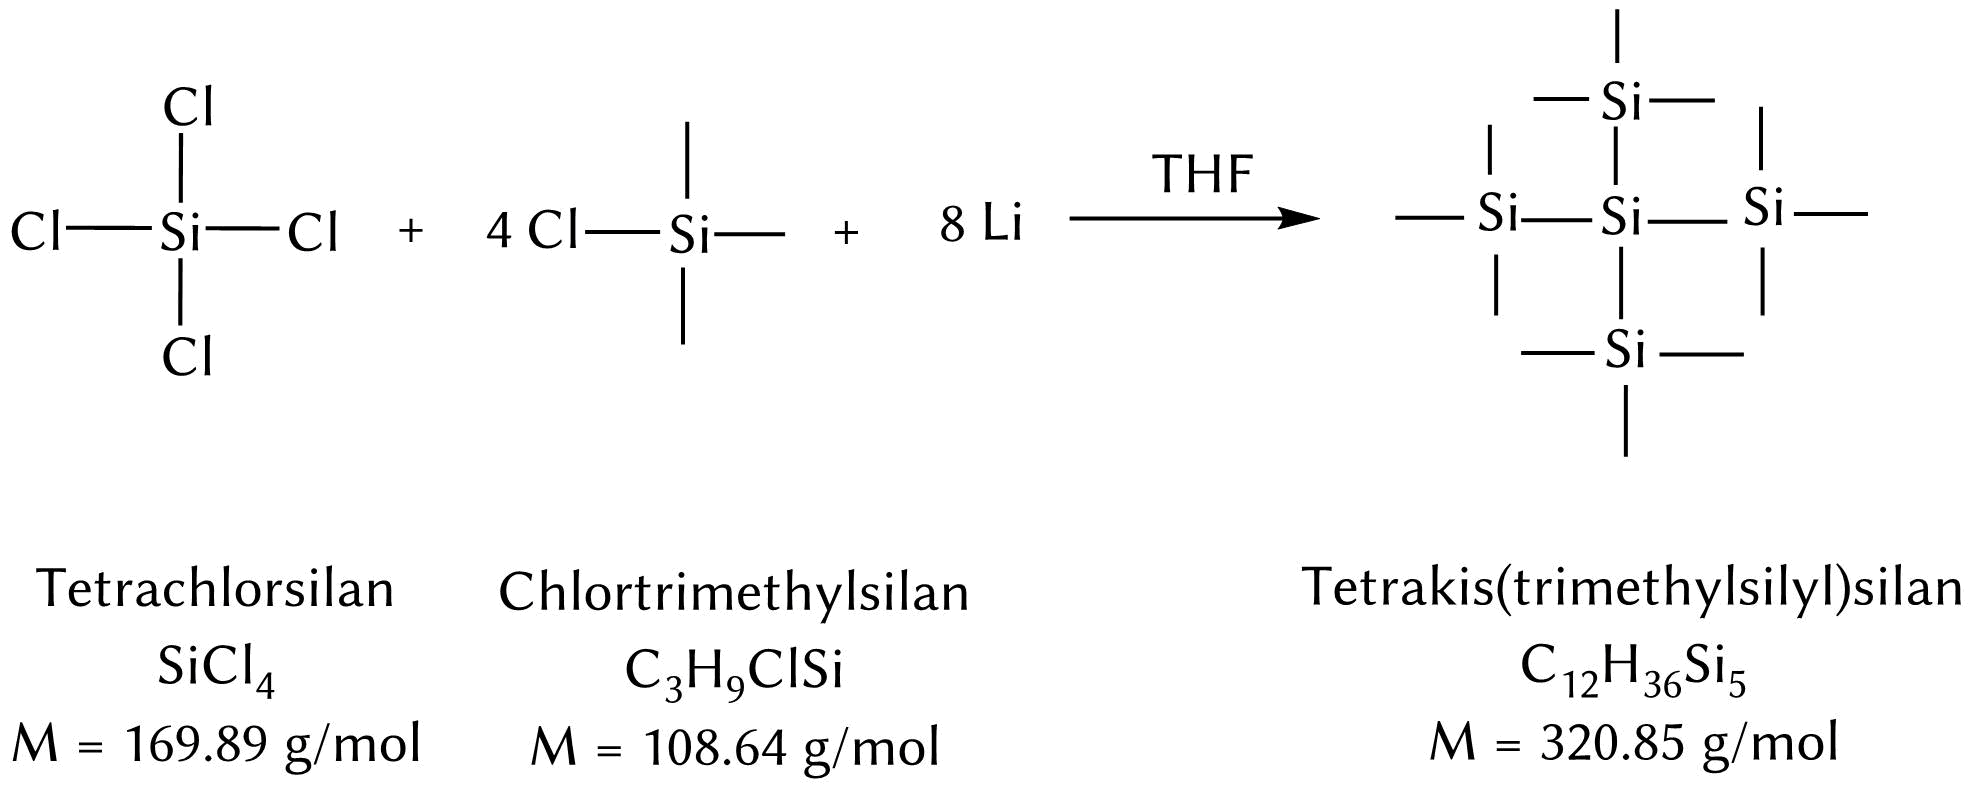
\includegraphics[width=\textwidth]{reaktion}
\end{scheme}

%\chemabove{\lewis{2:,Si}}{\hspace{5mm}\scriptstyle\ominus}
%%%%%%%%%%%%%
% Berechnung des Ansatzes
%%%%%%%%%%%%%
\begin{onehalfspace}

\section{Berechnung des Ansatzes: }
Es sollte 2,2-Diphenylpent-4-enylamin aus 2,2-Diphenylpent-4-ennitril (20.75 g, 88.9 mmol) hergestellt werden. Die Umrechnung des Literaturansatzes ergab folgenden Ansatz:\cite{bio}\\[0.5cm]
\begin{tabular}{lrrrr}
\toprule
\textbf{Bezeichnung }&\textbf{ M [\si{\gram\per\mol}]} & \textbf{n [\si{\milli\mol}]} & \textbf{Menge} & \textbf{Equiv}\\
\midrule
2,2-Diphenylpent-4-ennitril & 233.32 & 89  & 20.75 \si{\gram} & 1.00 \\
Lithiumaluminumhydrid  & 37.95   &  200  &  7.60 \si{\gram} & 2.24 \\
Diethylether &   & & 350  \si{\milli\liter}& LM \\
\bottomrule
\end{tabular}\\

%%%%%%%%%%%%%
% Durchführung
%%%%%%%%%%%%%
\normalsize \section{Durchführung \cite{vor}}
Zur Darstellung des 2,2-Diphenylpent-4-enylamin wurden in einem 500 ml-Schlenkkolben
Lithiumaluminumhydrid (7.60 \si{\gram}, 89 \si{\milli\mol}) in Diethylether (300 \si{\milli\liter}) vorgelegt und mit einem Eis-Kochsalz-Kältebad auf etwa -5 \si{\celsius} abgekühlt.
Zu dieser Suspension wurde 2,2-Diphenylpent-4-ennitril (20.75~\si{\gram}, 89 \si{\milli\mol}) in Diethylether (50 \si{\milli\liter}) zugetropft und
 bei Raumtemperatur 48~Stunden gerührt. Im Anschluss wurde die Suspension 30 Minuten lang unter Rückfluss zum Sieden erhitzt.
Nach dem die Apparatur auf die Raumtemperatur gekühlt worden war, wurde die Suspension auf ein Eisbad gestellt.
Der Überschuss an Lithiumaluminumhydrid wurde mit Wasser (100 \si{\milli\liter}) vorsichtig zerstört, wobei sich zwei Phasen bildete.
 Die klare etherische Phase wurde abdekantiert und die wässrige Phase wurde mit Diethylether (2 x 100 \si{\milli\liter}) extrahiert.
  Die vereinten etherischen Phasen wurden mit Magnesiumsulfat getrocknet
und in einen 500 ml-Kolben, ausgestattet mit Rückflusskühler, überführt.
Zur Freisetzung des Amins aus dem Ammoniumsalz wurden eine Natriumhydroxidlösung (10 \% ig,50~\si{\milli\liter}) und eine gesättigte
Kaliumsulfatlösung (100~\si{\milli\liter}) unter Kühlung im Eisbad zugetropft.
Die wässrige Phase wurde mit Diethylether (2 x 100 \si{\milli\liter}) extrahiert, mit Magnesiumsulfat getrocknet, das Lösungsmittel im Rotationsverdampfer entfernt und
 das Rohprodukt an der Hochvakuumpumpe getrocknet. Das Produkt (19.30 \si{\gram}, 81 \si{\milli\mol}, 91 \%) wurde als farblose Flüssigkeit erhalten.

%%%%%%%%%%%%
% Ausbeute
%%%%%%%%%%%%%
\section{Ausbeute}
\begin{tabular}{ ll}
  21.10 g (89 mmol)   & = 100 \%\\
  19.30 g (81 mmol)    & = 91 \% (Lit.\cite{vor} : 77 \%) \\
 \end{tabular}
\pagebreak
%%%%%%%%%%%%%
%Physikalische Daten des Produktes
%%%%%%%%%%%%%
%\section{Physikalische Daten des Produktes}
%\textit{2,2-Dimethyl-pent-4-enenitril}


\section{Spektrenauswertung}

\begin{scheme}[!ht]
   \centering
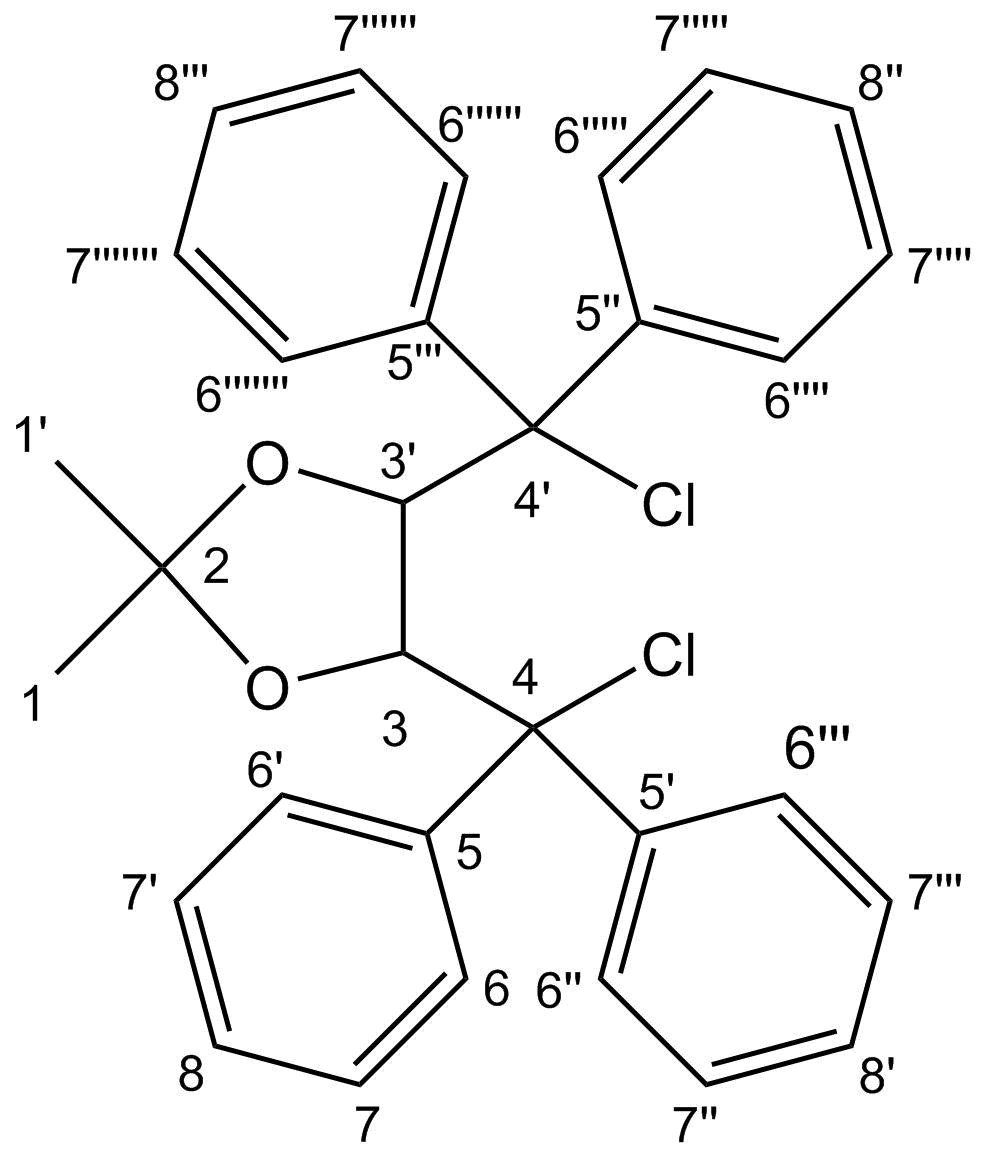
\includegraphics{auswert}
\end{scheme}

%\begin{experimental}[format=\bfseries,delta=(ppm),list=true,use-equal]
%\data{IR}[NaCl] \val{2935} (), \val{3061} (w)
%\hspace{5mm}
%\NMR* (300 \si{\MHz}, \ch{CDCl3}): \chemdelta =
%\val{3.06} (d, $^{3\!}\textit{J} = 15.9$ \si{\Hz}, \#{2}, \pos{3}),
%\val{5.05 -- 5.19 } (m, \#{2}, \pos{5}),
%\val{5.64} (ddt, $^{3\!}\textit{J} = 7$ \si{\Hz},$^{2\!}\textit{J} = 10.1$ \si{\Hz},$^{2\!}\textit{J} = 17.1$ \si{\Hz}, \#{1}, \pos{4}),
%\val{7.12 -- 7.50} (m, \#{10}, \pos{6}, \pos{7}, \pos{8}, \pos{9}) ppm.
%\end{experimental}
\noindent
\textbf{\ce{^1_{}H-NMR}} (300 MHz, \ce{CDCl_3}): \sffamily \ce{$\delta$} =
1.55 (s, 2 H, \ce{N-H}),
2.86 (d, \ce{^3_{}\textit{J}} = 7.0 \si{\hertz}, 2 H, 3-H),
3.27 (s, 2 H, 1-H),
5.06 – 4.80 (m, 2 H, 5-H),
5.40 – 5.20 (m, 1 H, 4-H),
7.17 – 6.98 (m, 10 H, 6-H, 7-H, 8-H, 9-H) ppm.\\

\noindent
\textbf{\ce{^1_{}H-NMR}} (500 MHz, \ce{CDCl_3}): \sffamily \ce{$\delta$} =
0.85 (s, 2 H, \ce{N-H}),
2.85 (d, \ce{^3_{}\textit{J}} = 7.1 \si{\hertz}, 1 H, 3-H),
3.25 (s, 2 H, 1-H),
4.86 - 5.01 (m, 2 H, 5-H),
5.32 (ddt, \ce{^3_{}\textit{J}} = 7.0~\si{\hertz}, \ce{^3_{}\textit{J}_{cis}} = 10.1 \si{\hertz}, \ce{^3_{}\textit{J}_{trans}} = 17.1 \si{\hertz}, 1 H, 4-H),
7.08 – 7.25 (m, 10 H, 6-H, 7-H, 8-H, 9-H) ppm. \\

\noindent
\textbf{\ce{^{13}_{}C-NMR}} (125 MHz, DEPT, \ce{CDCl_3}): \sffamily \ce{$\delta$} =
41.1 (\ce{CH2}, C-3),
48.5 (\ce{CH2}, C-1),
51.3 (C, C-2),
117.6 (\ce{CH2}, C-5),
126.0 (CH, C-9),
128.0 + 128.1 (2 x CH, C-7, C-8),
134.6 (CH, C-4),
146.2 (C, C-6) ppm.


\section{Mechanismus\cite{bio}}
Im ersten Schritt der Reaktion reagiert das nukleophile H-Atom des
Lithiumaluminiumhydrids (\textbf{2}) mit dem elektropilen Kohlenstoffatom des 2,2-Diphenylpent-4-ennitrils,
wobei sich ein Iminoaluminatsalz \textbf{3} bildet. Anschließend wird ein Wasserstoff intramolekular auf das C-Atom der Iminogruppe übertragen.
Das entstehende Salz \textbf{4} reagiert mit Wasser in einer Säure-Base-Reaktion.
Es bildet sich unter Abspaltung von \ce{LiOH} ein Aminoaluminiumhydrid \textbf{5}.
 Das Aminoaluminiumhydrid \textbf{5} wird ebenfalls hydrolysiert und
es bildet sich ein Aluminumhydridoammoniumsalz \textbf{6}. In einer mehrstufigen Reaktion werden die Hydroxyanionen an das Aluminumatom des Aluminumhydridoammoniumsalzes \textbf{6} addiert
und das gewünschte Produkt 2,2-Diphenylpent-4-enylamin (\textbf{7}) wird unter Abspaltung von \ce{Al(OH_3)} und \ce{H_2} freigesetzt.
\pagebreak
 \begin{scheme}[!ht]
   \centering
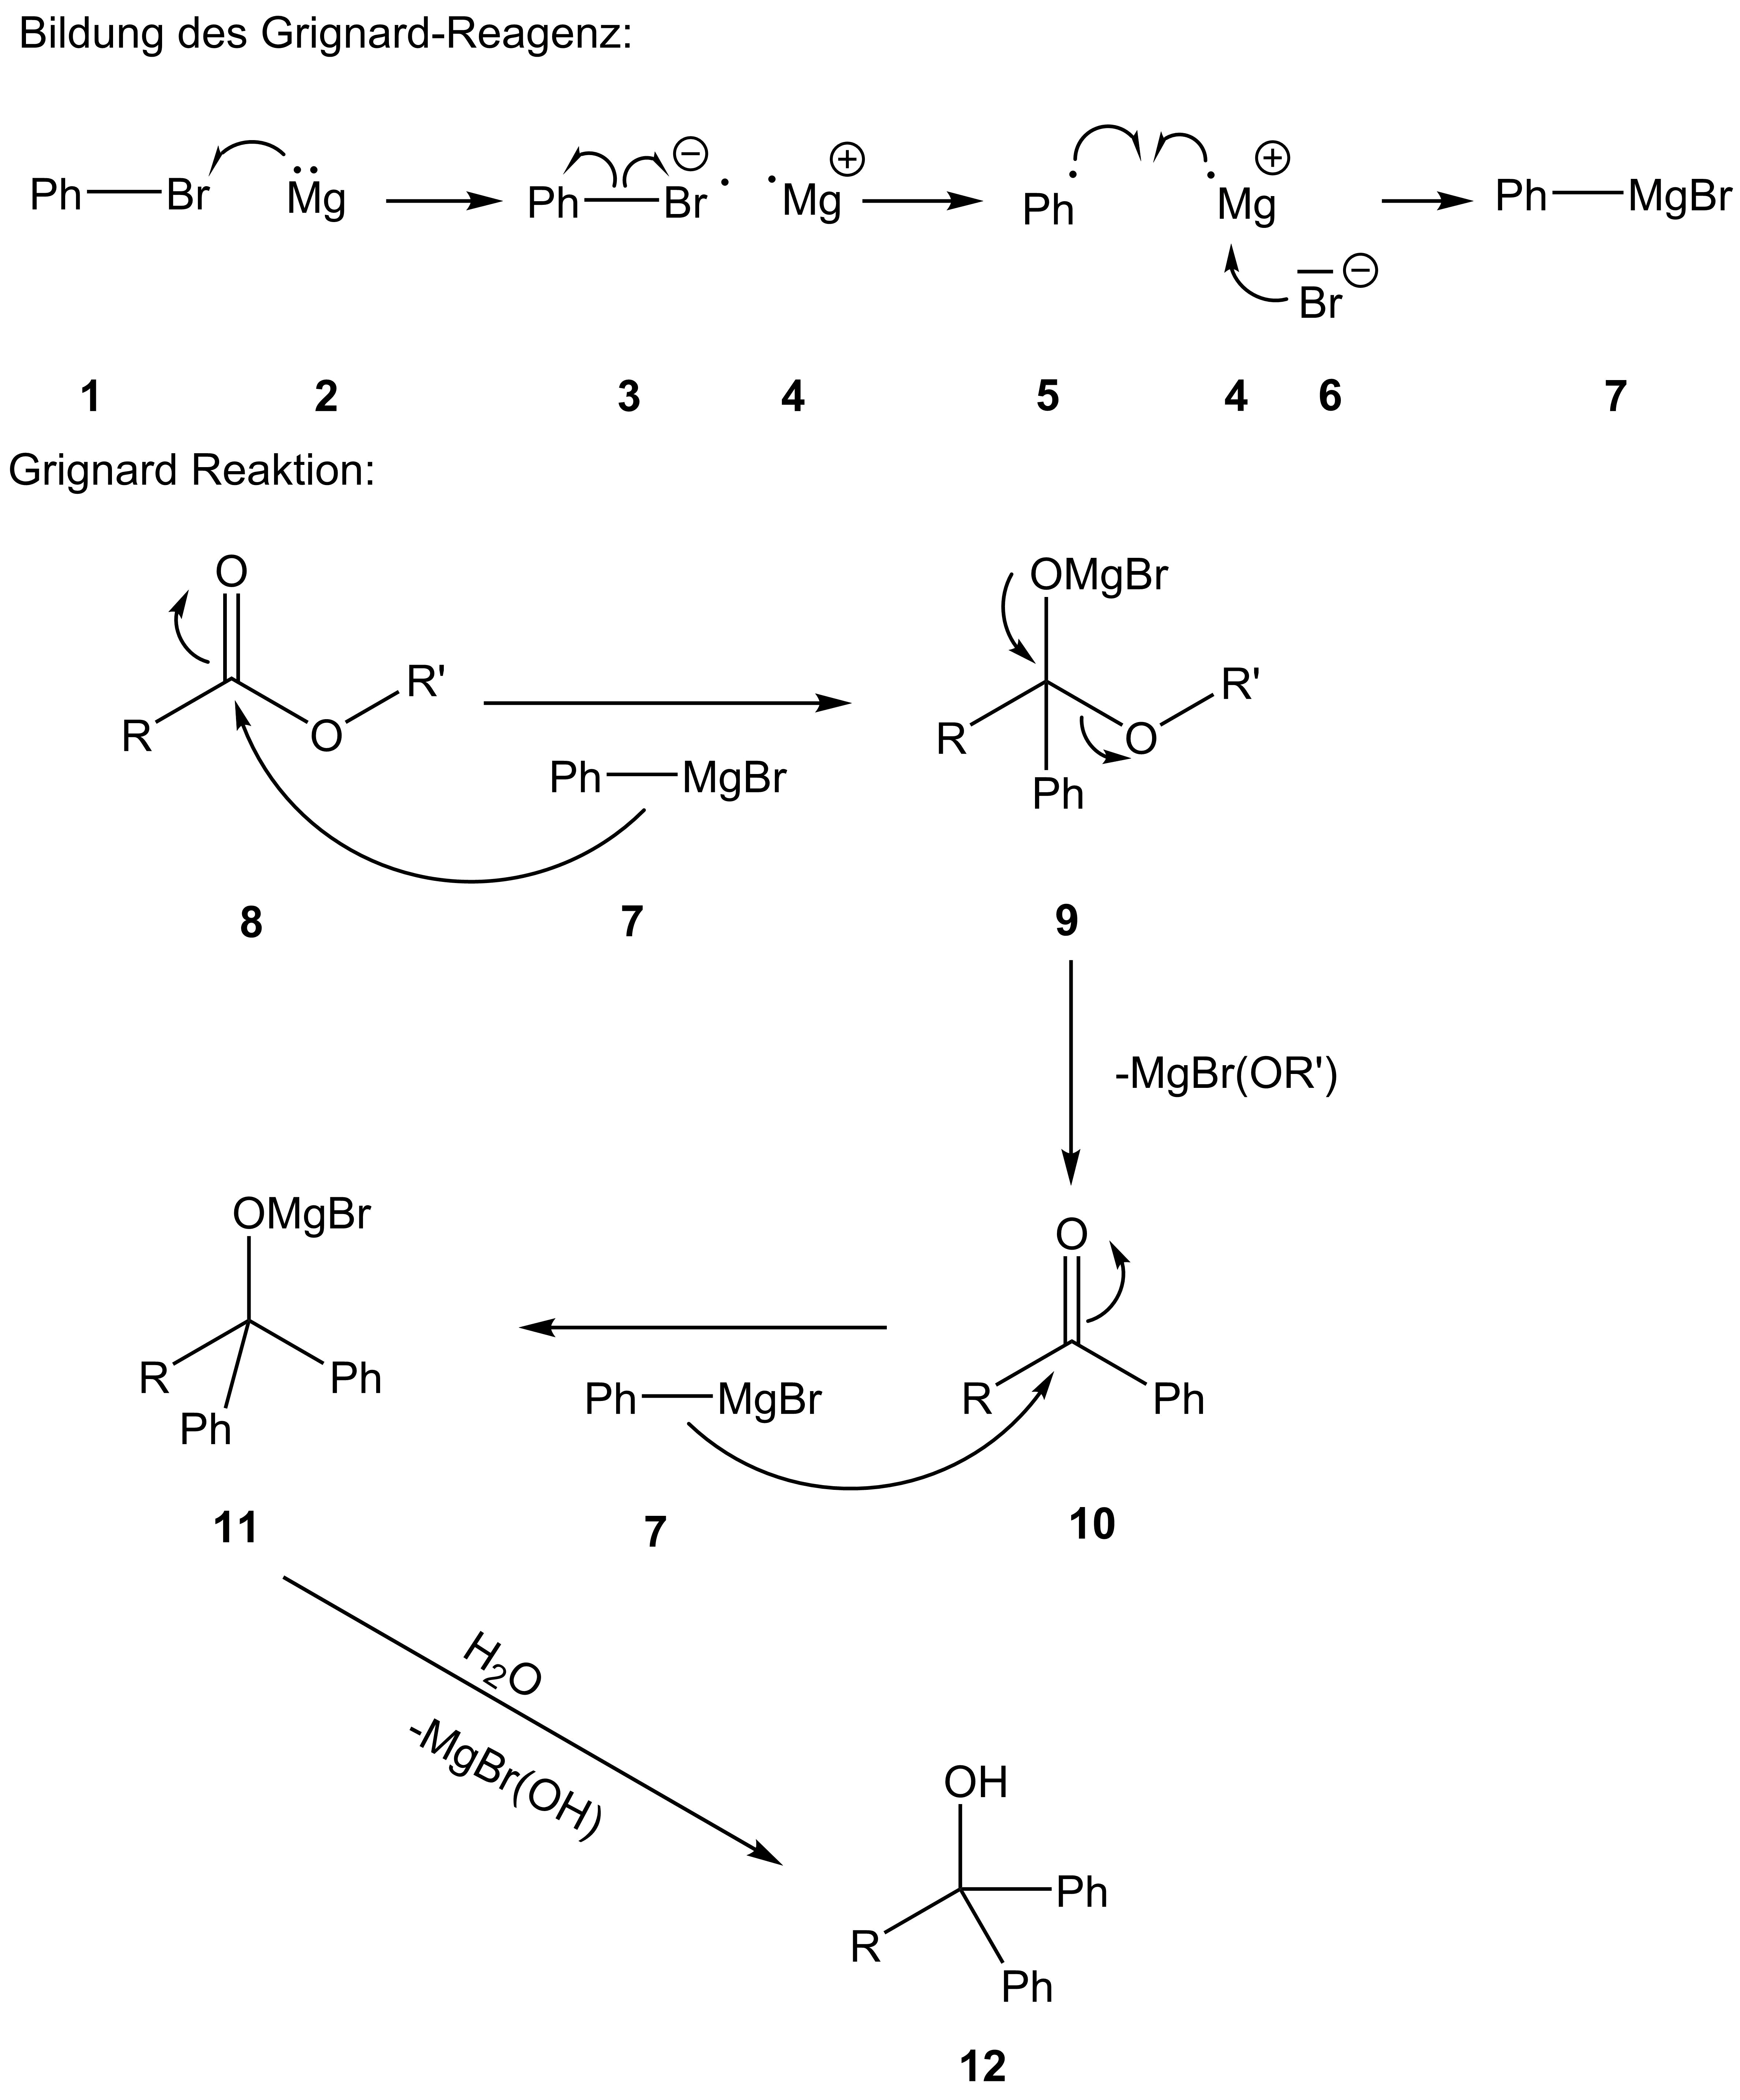
\includegraphics[width=\textwidth]{mechan}
\end{scheme}

\section{Abfallentsorgung}
Die nach dem Hydrolysieren verbleibenden wässrigen Phasen wurden
nach einer pH-Wertbestimmung im Behälter für basische wässrige Abfälle entsorgt.
Die nach dem Hydrolysieren ausgefallenen Lithium- und Aluminumsalze wurden in den Feststoffbehälter gegeben.
Das im Rotationsverdampfer abgetrennte Lösungsmittel wurde im Behälter für halogenfreie Kohlenwasserstoffe entsorgt.
\section{Literatur}
\renewcommand{\section}[2]{}%

\def\bibindent{0em}
\begin{thebibliography}{99\kern\bibindent}
\makeatletter
\let\old@biblabel\@biblabel
\def\@biblabel#1{\old@biblabel{#1}\kern\bibindent}
\let\old@bibitem\bibitem
\def\bibitem#1{\old@bibitem{#1}\leavevmode\kern-\bibindent}
\makeatother
\bibitem{vor}
P. Martinez, K. C. Hultzsch, F. Hampel, \textit{Chem. Commun.} \textbf{2006}, 2221 - 2223.
\bibitem{bio}
J. Buddrus, \textit{Grundlagen der Organische Chemie}, 4. Aufl., De Gruyter, Berlin \textbf{2011}, S. 532.
\end{thebibliography}
\end{onehalfspace}
\end{document}


